\section{Auswahl der Trainingsinfrastruktur}

cloud
rechenharware

Werden gängige Tesla GPUs, die Kunden als PaaS-Angebot zur Verfügung gestellt werden, nach ihrer Rechenleistung verglichen, so ergibt sich Tabelle \ref{gpus} \cite{TechPowerUp.20200209}.

\begin{center}
	\begin{tabular}[h]{l|c|c|c|c|c|c}
		& K80 & P100 & T4 & V100 & GTX 1080 & TITAN RTX \\
		\hline
		CUDA Cores & 2496 & 3584 & 2560 & 5120 & 2560 & 4608 \\
		Tensor Cores & / & / & 320 & 640 & / & 576 \\
		TeraFLOPS (Single Precision) & 4,113 & 9,526 & 8,141 & 14,13 & 8,873 & 16,31 \\
		Memory Bandwidth (in GB/sec) & 240,6 & 732,2 & 320 & 897 & 320,3 & 672 \\
		Suggested Power Supply Unit & 700 & 600 & 350 & 600 & 450 & 600
		\label{gpus}
	\end{tabular}
	\captionof{table}{Vergleich von GPUs nach Rechenleistung}
\end{center}

Auch wurden die Desktop-Grafikkarten \textit{GeForce GTX 1080} sowie die \textit{Titan RTX} in den Vergleich mit aufgenommen. Der Vergleich dient später dazu, um eine begründete Kosten-Nutzen Abwägung zwischen einem Trainieren der Modelle auf der Cloud oder lokal vollziehen zu können. 

Diese Art von Spezialhardware erreicht pro TPU-Kern eine Rechenleistung von bis zu 92 TOPS \cite{HaraldBogeholz.20170406}. Werden 2048 solcher TPU-Kerne zu einem TPU-Pod zusammen geschlossen, so ergibt sich eine Rechenleistung von über 100 PetaFLOPS \cite{GoogleCloud.20200209}. Zudem ist die größere Rechenleistung gleichzeitig effizienter als herkömmliche GPUs (siehe Abbildung \ref{tpu}).

\begin{figure}[ht]
	\begin{center}
		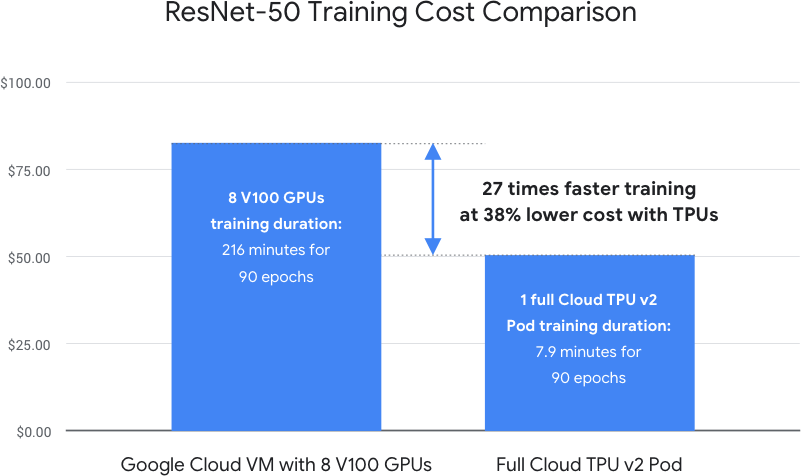
\includegraphics[width=14cm]{Bilder/tpu_comparison.png} 
		\caption[Vergleich V100 - TPU Pod]{Vergleich V100 - TPU Pod \cite{GoogleCloud.20200209b}}
		\label{tpu}
	\end{center}
\end{figure}

bild floydhub
gcp und amazon gibt sich nicht viel

FloydHub betreibt ein zeitbasiertes Zahlungsmodell. So kosten 10 Stunden Laufzeit auf einer K80 12\$, auf einer V100 bereits 42\$. Zusätzlich werden monatliche Account-Gebühren berechnet. Je nach Account kann eine unterschiedliche Anzahl an Projekten erstellt und Speicherplatz verwendet werden. Die \textit{Beginner} Ausstattung von einem Projekt und 10 GB Speicher ist allerdings kostenfrei. 